\subsection{二维随机变量}
\subsubsection{二维随机变量}
\paragraph{}
设$E$是一个随机试验,它的样本空间是$S=\{e\}$,设$X=X(e)$和$Y=Y(e)$是定义在$S$上的随机变量,由它们构成的一个向量$(X,Y)$,叫做\textbf{二维随机向量}或\textbf{二维随机变量}

\begin{figure}[h]
\centering
% 二维随机变量
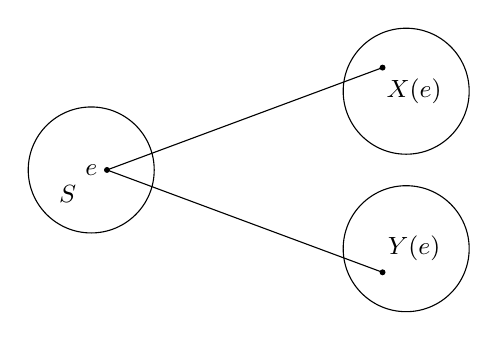
\begin{tikzpicture}
  % S = {e}
  \draw (0,0) circle [radius=0.8];
  \node at (0,0) {\small $e$};
  \node at (-0.3,-0.3) {\small $S$};

  % X = X(e)
  \draw (4,1) circle [radius=0.8];
  \node at (4.1,1) {\small $X(e)$};

  % Y = Y(e)
  \draw (4,-1) circle [radius=0.8];
  \node at (4.1,-1) {\small $Y(e)$};

  % 端点
  \draw [fill] (0.2,0) circle [radius=0.03];
  \draw [fill] (3.7,1.3) circle [radius=0.03];
  \draw [fill] (3.7,-1.3) circle [radius=0.03];
  % 连线
  \draw [thin] (0.2,0) -- (3.7,1.3);
  \draw [thin] (0.2,0) -- (3.7,-1.3);

\end{tikzpicture}

\caption{二维随机变量}
\label{二维随机变量}
\end{figure}

\paragraph{}
\textbf{定义\;}设$(X,Y)$是二维随机变量,对于任意实数$x,y$,二元函数:

\begin{equation}
  F(x,y) = P\{(X \leq x) \cap (Y \leq y) \} \xlongequal{\text{记成}} P\{X \leq x, Y \leq y\}
\end{equation}

称为二维随机变量$(X,Y)$的\textbf{分布函数},或称为随机变量$X$和$Y$的\textbf{联合分布函数}。

\paragraph{}

\begin{figure}[h]
\centering
  %------- 第1行 -------
  \begin{subfigure}[t]{0.48\linewidth}
    \centering
      % 二维随机变量的分布函数图解
\begin{tikzpicture}[scale = 0.9]
  \begin{axis}[clip=false,xmin=-1.5,xmax=4,ymin=-1.5,ymax=4,ticks=none,axis lines=middle,smooth,xlabel={$x$}, ylabel={$y$}]
    \draw (-1,3) -- (3,3) -- (3,-1);
    \fill[pattern=north east lines] (-1,-1) rectangle (3,3);
    \node[above] at (3,3) {$(x,y)$};
    \node[below left,fill=white, inner sep=1.5] at (0,0) {$O$};
  \end{axis}
\end{tikzpicture}

    \subcaption{分布函数图解}
  \end{subfigure}
  \begin{subfigure}[t]{0.48\linewidth}
    \centering
      % 二维随机变量的分布函数图解,矩形域
\begin{tikzpicture}[scale = 0.9]
  \begin{axis}[clip=false,xmin=-1.5,xmax=4,ymin=-1.5,ymax=4,ticks=none,axis lines=middle,smooth,xlabel={$x$}, ylabel={$y$}]
    % 矩形
    \draw (1,1) rectangle (3,3);
    % 矩形辅助线
    \draw[dashed] (0,3) -- (1,3);
    \node[left] at (0,3) {$y_2$};
    \draw[dashed] (0,1) -- (1,1);
    \node[left] at (0,1) {$y_1$};
    % 矩形辅助线
    \draw[dashed] (1,1) -- (1,0);
    \node[below] at (1,0) {$x_1$};
    \draw[dashed] (3,1) -- (3,0);
    \node[below] at (3,0) {$x_2$};
    % (x,y)
    \node[above] at (3,3) {$(x,y)$};
    % 原点
    \node[below left, inner sep=1.5] at (0,0) {$O$};
  \end{axis}
\end{tikzpicture}

    \subcaption{矩形域图解}
  \end{subfigure}
  \caption{分布函数图解}
  \label{二维随机变量的分布函数图解}
\end{figure}

\textbf{性质:\;}

\begin{enumerate}
  \item $F(x,y)$是变量$x$和$y$的不减函数,即对于任意固定的$y$,当$x_2 > x_1$时$F(x_2,y)\geq F(x_1,y)$;对于任意固定的$x$,当$y_2 > y_1$时$F(x,y_2) \geq F(x,y_1)$。
  \item $0 \leq F(x,y) \leq 1$,且
  \begin{enumerate}
    \item 对于任意固定的$y, F(-\infty,y)=0$,
    \item 对于任意固定的$x, F(x,-\infty)=0$,
    \item $F(-\infty, -\infty) = 0, F(\infty,\infty)=1$。
  \end{enumerate}
  \item $F(x+0,y)=F(x,y),F(x,y+0)=F(x,y)$,即$F(x,y)$关于$x$右连续,关于$y$也右连续。
  \item 对于任意$(x_1,y_1), (x_2,y_2), x_1 < x_2, y_1 < y_2$,下述不等式成立:
  \begin{equation}
    F(x_2,y_2) - F(x_2,y_1) + F(x_1,y_1) - F(x_1,y_2) \geq 0.
  \end{equation}
  参考\linkref[二维随机变量的分布函数图解]{矩形域图解}。
\end{enumerate}

\subsubsection{离散型的随机变量}
\paragraph{}
如果二维随机变量$(X,Y)$全部可能取到的值是\textbf{有限对}或\textbf{可列无限多对},则称$(X,Y)$是\textbf{离散型的随机变量}。
\paragraph{}
设二维离散型随机变量$(X,Y)$所有可能取的值为$(x_i,y_j),i,j=1,2,\cdots,$记$P\{X=x_i,Y=y_j\}=p_{ij},i,j=1,2,\cdots,$则由概率的定义有

\begin{equation}
  p_{ij} \geq 0, \sum_{i=1}^\infty\sum_{j=1}^\infty p_{ij} = 1.
\end{equation}

\paragraph{}
我们称$P\{X=x_i,Y=y_j\}=p_{ij},i,j=1,2,\cdots$为二维离散型随机变量$(X,Y)$的\textbf{分布律},或随机变量$X$和$Y$的\textbf{联合分布律}。

\paragraph{}
我们也能用表格来表示$X$和$Y$的联合分布律:

\bgroup
\def\arraystretch{1.5}
\setlength\tabcolsep{0.8cm}
\begin{figure}[H]
\centering
  \begin{tabular}{c|ccccc}
    \hline
    \backslashbox{$Y$}{$X$} & $x_1$ & $x_2$ & $\cdots$ & $x_i$ & $\cdots$ \\
    \hline
    $y_1$ & $p_{11}$ & $p_{21}$ & $\cdots$ & $p_{i1}$ & $\cdots$ \\
    \hline
    $y_2$ & $p_{12}$ & $p_{22}$ & $\cdots$ & $p_{i2}$ & $\cdots$ \\
    \hline
    $\vdots$ & $\vdots$ & $\vdots$ &  & $\vdots$ & \\
    \hline
    $y_j$ & $p_{1j}$ & $p_{2j}$ & $\cdots$ & $p_{ij}$ & $\cdots$ \\
    \hline
    $\vdots$ & $\vdots$ & $\vdots$ &  & $\vdots$ & \\
    \hline
  \end{tabular}
\end{figure}
\egroup

\paragraph{}
将$(X,Y)$看成一个随机点的坐标,由图\figureref{二维随机变量的分布函数图解}知道离散型随机变量$X$和$Y$的\textbf{联合分布函数}为:

\begin{equation}
  \label{离散型随机变量的联合分布函数}
  F(x,y) = \sum_{x_i \leq  x} \sum_{y_j \leq y} p_{ij},
\end{equation}

其中和式是对一切满足$x_i \leq x, \; y_j \leq y$的$i,j$来求和的。

\subsubsection{连续型的随机变量}
\paragraph{}
对于二维变量$(X,Y)$的分布函数$F(x,y)$,如果存在非负的函数$f(x,y)$使对于任意$x,y$有

\begin{equation}
  F(x,y)=\int_{-\infty}^y\int_{-\infty}^xf(u,v)dudv,
\end{equation}

则称$(X,Y)$是\textbf{连续型的二维随机变量},函数$f(x,y)$称为二维随机变量$(X,Y)$的\textbf{概率密度},或称为随机变量$X$和$Y$的\textbf{联合概率密度}。

\paragraph{}
概率密度$f(x,y)$具有以下性质:
\begin{enumerate}
  \item $f(x,y) \geq 0$
  \item $\int_{-\infty}^\infty\int_{-\infty}^\infty f(x,y)dxdy=F(\infty,\infty)=1$
  \item 设$G$是$xOy$平面上的区域,点$(X,Y)$落在$G$内的概率为
  \begin{equation}
    P\{(X,Y)\in G\} = \iint\limits_G f(x,y)dxdy
  \end{equation}
  \item 若$f(x,y)$在点$(x,y)$连续,则有
  \begin{equation}
    \frac{\partial^2F(x,y)}{\partial x\partial y} = f(x,y)
  \end{equation}
\end{enumerate}

\subsubsection{$n$维随机变量}
\paragraph{}
一般,设$E$是一个随机试验,它的样本空间是$S=\{e\}$,设$X_1=X_1(e), X_2=X_2(e),\cdots,X_n=X_n(e)$是定义在$S$上的随机变量,由它们构成的一个$n$维向量$(X_1,X_2,\cdots,X_n)$叫做\textbf{$n$维随机向量}或\textbf{$n$维随机变量}。
\paragraph{}
对于任意$n$个实数$x_1,x_2,\cdots,x_n$,$n$元函数
\begin{equation}
  F(x_1,x_2,\cdots,x_n)=P\{X_1 \leq  x_1, X_2 \leq x_2, \cdots, X_n \leq x_n\}
\end{equation}
称为$n$维随机变量$(X_1,X_2,\cdots,X_n)$的\textbf{分布函数}或随机变量$X_1,X_2,\cdots,X_n$的\textbf{联合分布函数}。它具有类似于二维随机变量的分布函数的性质。

\subsection{边缘分布}
\subsubsection{边缘分布}
\paragraph{}
二维随机变量$(X,Y)$作为一个整体,具有分布函数$F(x,y)$,而$X$和$Y$都是随机变量,各自也有分布函数,将它们分别记为$F_X(x), F_Y(y)$,依次称为二维随机变量$(X,Y)$关于$X$和关于$Y$的\textbf{边缘分布函数},边缘分布函数可以由$(X,Y)$的分布函数$F(x,y)$所确定,事实上,
\begin{equation}
  F_x(x) = P\{X\leq x\} = P\{X\leq x, Y < \infty\} = F(x,\infty),
\end{equation}
即
\begin{equation}
  \label{F_X(x)边缘分布}
  F_X(x)=F(x,\infty).
\end{equation}
就是说,只要在函数$F(x,y)$中令$y \to \infty$就能得到$F_X(x)$,同理
\begin{equation}
  F_Y(y) = F(\infty,y).
\end{equation}

\subsubsection{离散型随机变量}
\paragraph{}
对于离散型随机变量,由\eqref{离散型随机变量的联合分布函数}、\eqref{F_X(x)边缘分布}式可得
\begin{equation}
  F_X(x)=F(x,\infty)=\sum_{x_i \leq x}\sum_{j=1}^\infty p_{ij}.
\end{equation}

与第二章\eqref{X的分布函数}式比较,知道$X$的分布律为

\begin{equation}
  P\{X=x_i\} = \sum_{j=1}^\infty p_{ij}, \; i = 1, 2, \cdots.
\end{equation}

同样,$Y$的分布律为

\begin{equation}
  P\{Y=y_i\} = \sum_{i=1}^\infty p_{ij}, \; j = 1, 2, \cdots.
\end{equation}

记
\begin{align}
\begin{split}
  p_{i\bigcdot} &= \sum_{j=1}^\infty p_{ij} = P\{X=x_i\}, \; i = 1,2,\cdots, \\
  p_{\bigcdot j} &= \sum_{i=1}^\infty p_{ij} = P\{Y=y_j\}, \; j = 1,2,\cdots,
\end{split}
\end{align}

分别称$p_{i\bigcdot}(i=1,2,\cdots)$和$p_{\bigcdot j}(j=1,2,\cdots)$为$(X,Y)$关于$X$和关于$Y$的\textbf{边缘分布律}

\subsubsection{连续型随机变量}
\paragraph{}
对于连续型随机变量$(X,Y)$,设它的概率密度为$f(x,y)$,由于
\begin{equation}
  F_X(x) = F(x,\infty)=\int_{-\infty}^x\Big[\int_{-\infty}^\infty f(x,y)dy\Big]dx,
\end{equation}
由第二章\eqref{连续型随机变量的分布函数}式知道,$X$是一个连续型随机变量,且其概率密度为
\begin{equation}
  f_X(x) = \int_{-\infty}^\infty f(x,y)dy.
\end{equation}
同样,$Y$也是一个连续型随机变量,其概率密度为
\begin{equation}
  f_Y(y) = \int_{-\infty}^\infty f(x,y)dy.
\end{equation}
分别称$f_X(x),f_Y(y)$为$(X,Y)$关于$X$和关于$Y$的\textbf{边缘概率密度}。

\paragraph{}
平时将边缘分布律写在联合分布律表格的边缘上,这就是“边缘分布律”的由来,例如:

\bgroup
\def\arraystretch{1.5}
\setlength\tabcolsep{0.5cm}
\begin{figure}[H]
\centering
  \begin{tabular}{c|cccc|c}
    \hline
    \backslashbox{$F$}{$D$} & $1$ & $2$ & $3$ & $4$ & $P\{F=j\}$ \\
    \hline
    $0$ & $\frac{1}{10}$ & $0$ & $0$ & $0$ & $\frac{1}{10}$ \\
    $1$ & $0$ & $\frac{4}{10}$ & $\frac{2}{10}$ & $\frac{1}{10}$ & $\frac{7}{10}$ \\
    $2$ & $0$ & $0$ & $0$ & $\frac{2}{10}$ & $\frac{2}{10}$ \\
    \hline
    $P\{D=i\}$ & $\frac{1}{10}$ & $\frac{4}{10}$ & $\frac{2}{10}$  & $\frac{3}{10}$ & $1$ \\
    \hline
  \end{tabular}
\end{figure}
\egroup

即有边缘分布律
\bgroup
\def\arraystretch{2}
\setlength\tabcolsep{0.5cm}
\begin{figure}[H]
\centering
%------- 第1行 -------
\begin{subfigure}[t]{0.48\linewidth}
  \centering
    \begin{tabular}{c|cccc}
      \hline
      $D$ & $1$ & $2$ & $3$ & $4$ \\
      \hline
      $p_k$ & $\frac{1}{10}$ & $\frac{4}{10}$ & $\frac{2}{10}$ & $\frac{3}{10}$ \\
      \hline
    \end{tabular}
\end{subfigure}
\begin{subfigure}[t]{0.48\linewidth}
  \centering
    \begin{tabular}{c|ccc}
      \hline
      $F$ & $0$ & $1$ & $2$ \\
      \hline
      $p_k$ & $\frac{1}{10}$ & $\frac{7}{10}$ & $\frac{2}{10}$ \\
      \hline
    \end{tabular}
\end{subfigure}
\end{figure}
\egroup

\subsection{条件分布}
\subsubsection{离散型随机变量}
\paragraph{}
\textbf{定义\;}设$(X,Y)$是二维离散型随机变量,对于固定的$j$,若$P\{Y=y_j\}>0$,则称
\begin{equation}
  P\{X=x_i|Y=y_j\} = \frac{P\{X=x_i,Y=y_j\}}{P\{Y=y_j\}} = \frac{p_{ij}}{p_{\bigcdot j}}, \; i = 1,2,\cdots
\end{equation}
为在$Y=y_j$条件下随机变量$X$的\textbf{条件分布律}。同样,可得到$Y$的条件分布律。

\subsubsection{连续型随机变量}
\paragraph{}
\textbf{定义\;}设二维随机变量$(X,Y)$的概率密度为$f(x,y), (X,Y)$关于$Y$的边缘概率密度为$f_Y(y)$,若对于固定的$y, f_Y (y)>0$,则称$\frac{f(x,y)}{f_Y(y)}$为在$Y=y$的条件下$X$的\textbf{条件概率密度},记为
\begin{equation}
  f_{X|Y}(x|y) = \frac{f(x,y)}{f_Y(y)}.
\end{equation}

称$\int_{-\infty}^x f_{X|Y}(x|y)dx = \int_{-\infty}^x \frac{f(x,y)}{f_Y(y)}dx$为在$Y=y$的条件下$X$的条件分布函数,记为$P\{X \leq  x | Y = y\}$或$F_{X|Y}(x|y)$,即

\begin{equation}
  F_{X|Y}(x|y) = P\{X \leq x | Y = y\}=\int_{-\infty}^x\frac{f(x,y)}{f_Y(y)}dx.
\end{equation}

类似地,可以定义$f_{Y|X}(y|x)=\frac{f(x,y)}{f_X(x)}$和$F_{Y|X}(y|x)=\int_{-\infty}^y\frac{f(x,y)}{f_X(x)}dy.$

\subsection{相互独立的随机变量}
\paragraph{}
\textbf{定义\;}设$F(x,y)$及$F_X(x),F_Y(y)$分别是二维随机变量$(X,Y)$的分布函数及边缘分布函数。若对于所有$x,y$有
\begin{equation}
  P\{X \leq x, Y \leq y\} = P\{X \leq x\}P\{Y \leq y\},
\end{equation}
即
\begin{equation}
  \label{二维随机变量的相互独立性}
  F(x,y) = F_X(x)F_Y(y),
\end{equation}
则称随机变量$X$和$Y$是\textbf{相互独立的}。

\paragraph{}
设$(X,Y)$是连续型随机变量,$f(x,y), f_X(x), f_Y(y)$分别为$(X,Y)$的概率密度和边缘概率密度,则$X$和$Y$相互独立的条件\eqref{二维随机变量的相互独立性}等价于
\begin{equation}
  f(x,y)=f_X(x)f_Y(y)
\end{equation}
在平面上几乎处处成立。

\paragraph{}
当$(X,Y)$是离散型随机变量时,$X$和$Y$相互独立的条件\eqref{二维随机变量的相互独立性}式等价于:对于$(X,Y)$的所有可能取的值$(x_i,y_j)$有
\begin{equation}
  P\{X=x_i,Y=y_j\} = P\{X=x_i\}P\{Y=y_j\}.
\end{equation}

\textbf{定理\;}设$(X_1, X_2, \cdots, X_m)$和$(Y_1, Y_2, \cdots, Y_n)$相互独立,则$X_i(i=1,2, \cdots, m)$和$Y_j(j=1,2, \cdots, n)$相互独立,又若$h,g$是连续函数,则$h(X_1,X_2, \cdots, X_m)$和$g(Y_1, Y_2, \cdots, Y_n)$相互独立。
